
\section{OpenGL}

\begin{figure}[hbp]
\centering

\includegraphics[width=0.7\textwidth]{images/openGL/OpenGL_logo.jpg}
\end{figure}


\textbf{OpenGL} (“Open Graphics Library”) è una specifica che definisce un'\textbf{API} che fornisce metodi per sviluppare applicazioni di grafica 2D e 3D \cite{opengl-wiki}. E' stata introdotta nel 1992 dalla società californiana \textbf{Silicon Graphics}, è nata in ambiente Unix e, successivamente, è stata resa multipiattaforma. La libreria OpenGL è usata per vari tipi di applicazioni, come animazioni, videogiochi, simulazioni 3D e di realtà virtuale.

Una specifica è un documento che descrive un insieme di funzioni ed il comportamento preciso che queste devono avere. I maggiori produttori hardware (Nvidia, AMD, Intel, etc) creano implementazioni di queste funzioni rispettando la specifica OpenGL, usando l'accelerazione hardware quando possibile. In questo modo il programmatore può usufruire di un'API unificata, utilizzando le funzioni senza preoccuparsi della loro implementazione.

Un'altra caratteristica fondamentale è che le funzioni di OpenGL devono essere sempre usufruibili, quindi le implementazioni richiedono un'emulazione software quando l'hardware non è in grado di fornire certe funzionalità.

\subsection{Il funzionamento di OpenGL}
OpenGL offre circa 250 chiamate di funzione per disegnare scene a due  o tre dimensioni, a partire da delle primitive. Con primitive si intendono punti, linee e poligoni, i quali vengono convertiti in pixel tramite una serie di processi chiamata pipeline grafica.
La pipeline rappresenta una catena di trasformazioni e operazioni, in cui ogni fase prende in input il risultato della fase precedente e produce l'output per la fase successiva.

OpenGL opera a basso livello e richiede al programmatore di rispettare i passi precisi della pipeline che servono a renderizzare la scena. Tra i passi principali da seguire sono presenti :

\begin{itemize}
\item fornire le primitive che descrivano la scena.
\item fornire le regole per generare una telecamera virtuale, che renderizzi solo determinate porzione della scena, con particolari modalità.
\item fornire le regole per gestire texture, materiali, luci e ombre.
\end{itemize}

Queste regole vanno definite in particolari file chiamati \textbf{shader}, scritti in un linguaggio ad alto livello proprio di OpenGL, basato sul linguaggio C, chiamato \textit{GLSL} (“OpenGL Shading Language”). Siccome la scena non può essere renderizzata senza aver fornito le regole basilari, è necessaria, da parte del programmatore, una buona conoscenza della suddetta pipeline grafica e del linguaggio GLSL.

Esistono anche framework che operano ad alto livello, i quali nascondono al programmatore le fasi più complesse del rendering, gestendole autonomamente, e che richiedono solamente una descrizione generica della scena. Un'esempio è il framework Ogre3D, trattato più avanti.

\subsection{Le trasformazioni}

Nella figura \ref{pipeline} si possono vedere le principali fasi della pipeline.

\begin{figure}[htbp]
\centering
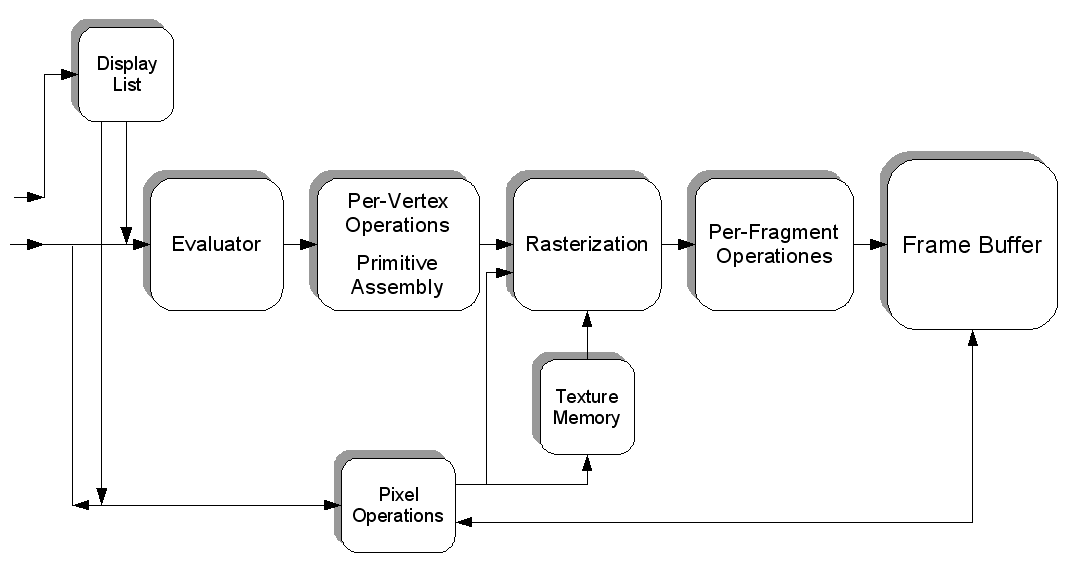
\includegraphics[width=0.7\textwidth]{images/frustum/opengl-pipeline.png}
\caption{La pipeline grafica.\label{pipeline}}
\end{figure}

Ai fini di questo progetto, ci concentreremo sulle trasformazioni, più che su altre operazioni come la \textbf{rasterizzazione} \footnote{Conversione da immagine vettoriale a bitmap (cioè da vettori a pixel), costruendo segmenti o porzioni di piano che riempiono lo spazio definito da due o più vertici.} o l'applicazione di materiali e texture.


Il diagramma in figura \ref{trans-pipe} mostra le principali trasformazioni eseguite nella pipeline.

\begin{figure}[htbp]
\centering
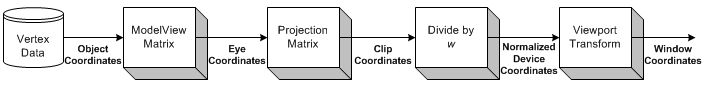
\includegraphics[width=0.7\textwidth]{images/frustum/transform-pipeline.png}
\caption{Le trasformazioni.\label{trans-pipe}}
\end{figure}

\subsubsection{Il sistema di coordinate in OpenGL}
Per determinare la posizione di ciascun vertice all'interno del mondo virtuale, viene adottato un sistema di coordinate a 3 dimensioni (figura \ref{cartesian}).
\begin{figure}[htbp]
\centering
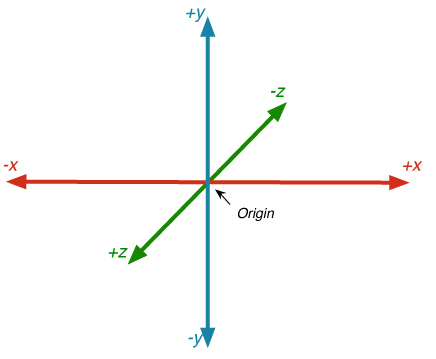
\includegraphics[width=0.4\textwidth]{images/frustum/cartesian.png}
\caption{Il sistema cartesiano in OpenGL e Ogre3D.\label{cartesian}}
\end{figure}
Da notare l'asse Z, la cui direzione positiva è quella uscente, ovvero quella rivolta verso l'utente che sta di fronte allo schermo. Questa caratteristica è fondamentale perchè determina il segno di alcuni elementi nel processo di trasformazione. 

Si considera che la telecamera virtuale \footnote{Con telecamera virtuale si intende tutto l'insieme di trasformazioni che renderizza una determinata porzione di spazio, come se la scena fosse inquadrata da una telecamera vera.} sia posizionata nell'origine del sistema, ovvero nel punto $(0,0,0)$, e che punti lo sguardo verso la direzione negativa dell'asse Z; gli assi X e Y sono paralleli al piano che rappresenta lo schermo (figura \ref{cam-default}).

\begin{figure}[htbp]
\centering
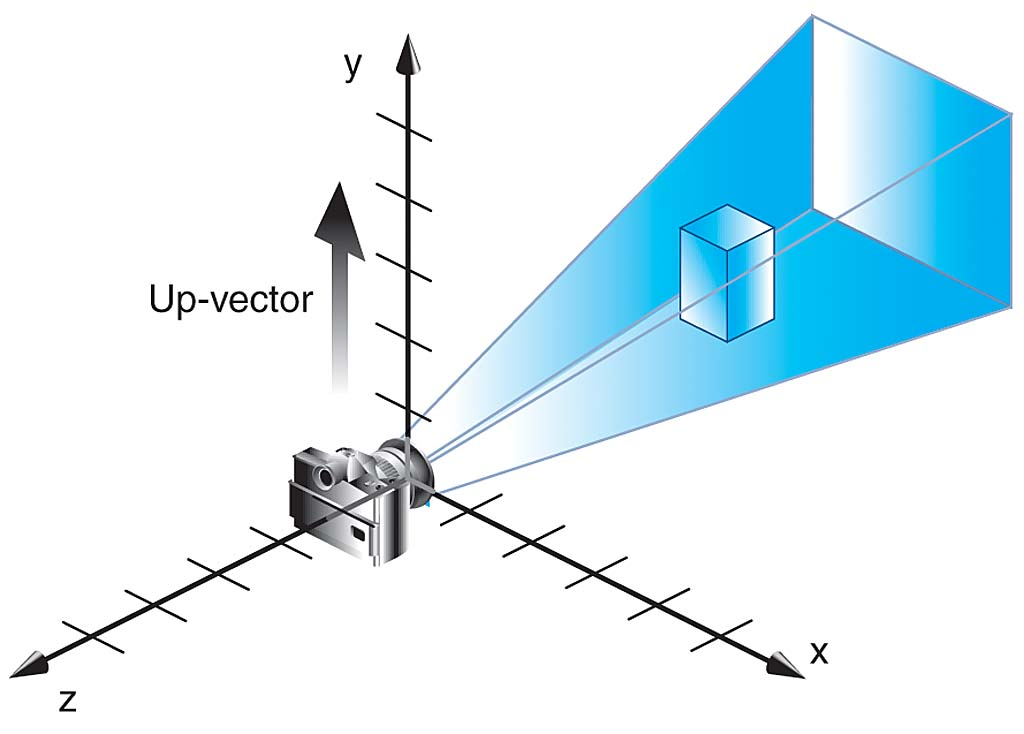
\includegraphics[width=0.5\textwidth]{images/frustum/camera-default.jpg}
\caption{La posizione di default della telecamera virtuale.\label{cam-default}}
\end{figure}

La porzione di spazio che viene inquadrata è definita “view volume” o \textbf{frustum} \footnote{“Tronco di piramide”. Per convenzione viene definito “frustum” anche quando assume la forma di un parallelepipedo (nella proiezione ortogonale).} (figura \ref{view-frustum}). 
\begin{figure}[htbp]
\centering
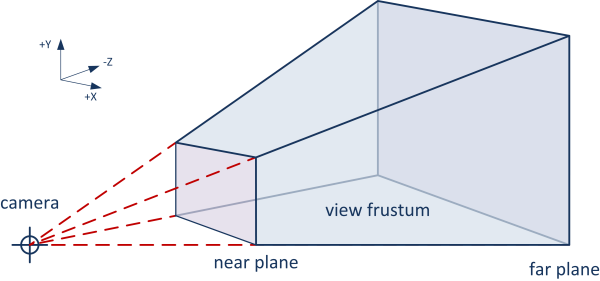
\includegraphics[width=0.5\textwidth]{images/frustum/view_frustum.png}
\caption{Il view volume nella proiezione prospettica.\label{view-frustum}}
\end{figure}
Il frustum è racchiuso da sei piani:
\begin{itemize}
\item \textit{near} e \textit{far plane}: sono i piani di inizio e fine scena.
\item \textit{left} e \textit{right plane}: sono i piani che racchiudono i bordi laterali.
\item \textit{bottom} e \textit{top plane}: sono i piani che racchiudono i bordi inferiore e superore.
\end{itemize}

Tutto ciò che è presente all'interno del frustum viene renderizzato a schermo; il resto non viene considerato.

\subsubsection{Model Matrix}
Nel prima fase si utilizza una matrice chiamata \textbf{Model Matrix}, che trasforma le coordinate locali degli oggetti presenti nella scena nel sistema globale di coordinate relativo al mondo virtuale. 

\subsubsection{Projection Matrix}

%
%Questo spazio è caratterizzato da un piano più vicino alla telecamera, il near plane, e uno più lontano, il far plane. Il near plane rappresenta la coordinata Z dalla quale sarà renderizzata la scena, ovvero tutto ciò che sta dietro non sarà visibile. Il far plane rappresenta la coordinata Z di fine scena, perciò determina quanto in profondità essa è visibile.

La \textbf{Projection Matrix} ha il compito di trasformare il frustum in un cubo $2\times2\times2$, centrato nell'origine, determinando anche la trasformazione di tutto ciò che è presente al suo interno. Ogni vertice all'interno di esso avrà coordinate $-1\leq x,y,z \leq 1$. Questo nuovo sistema di riferimento è chiamato \textbf{NDC}, “Normalized Device Coordinates”, mentre la porzione di spazio definita dal cubo ora prende il nome di \textbf{canonical view volume}.

Il modo in cui viene identificato il frustum, e quindi il modo in cui viene trasformato lo spazio, dipende dal tipo di proiezione. Essenzialmente esistono due tipi di proiezione, quella ortogonale e quella prospettica.

\begin{figure}[htbp]
\centering
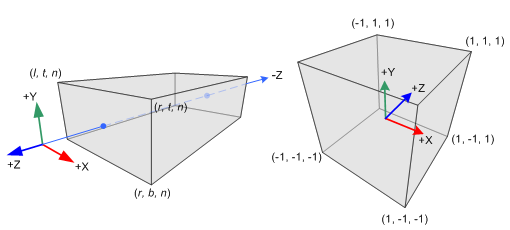
\includegraphics[width=0.5\textwidth]{images/frustum/orto-projection.png}
\caption{Trasformazione con proiezione ortogonale.\label{orto}}
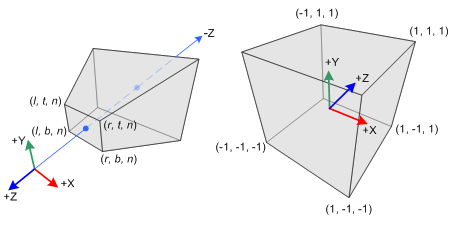
\includegraphics[width=0.5\textwidth]{images/frustum/persp-projection.png}
\caption{Trasformazione con proiezione prospettica.\label{persp}}
\end{figure}

In quella ortogonale (figura \ref{orto}) il frustum è rappresentato da un parallelepipedo; in questo caso tutti i vertici vengono proiettati sul near plane, parallelamente alla direzione della telecamera. Il risultato sarà quello di avere una visione non prospettica della scena.

Nella proiezione prospettica il frustum assume la forma di un tronco di piramide.
Il vertice della piramide è dato dalla posizione della telecamera, mentre il near plane e il far plane sono rispettivamente la base minore e maggiore del frustum. Dopo aver applicato questa trasformazione, il frustum diventerà un cubo, e tutti gli oggetti al suo interno saranno deformati per come sono visti a schermo.

Nelle figure \ref{example1} e \ref{example2} è possibile vedere un esempio di questa trasformazione.
\begin{figure}[htbp]
\centering
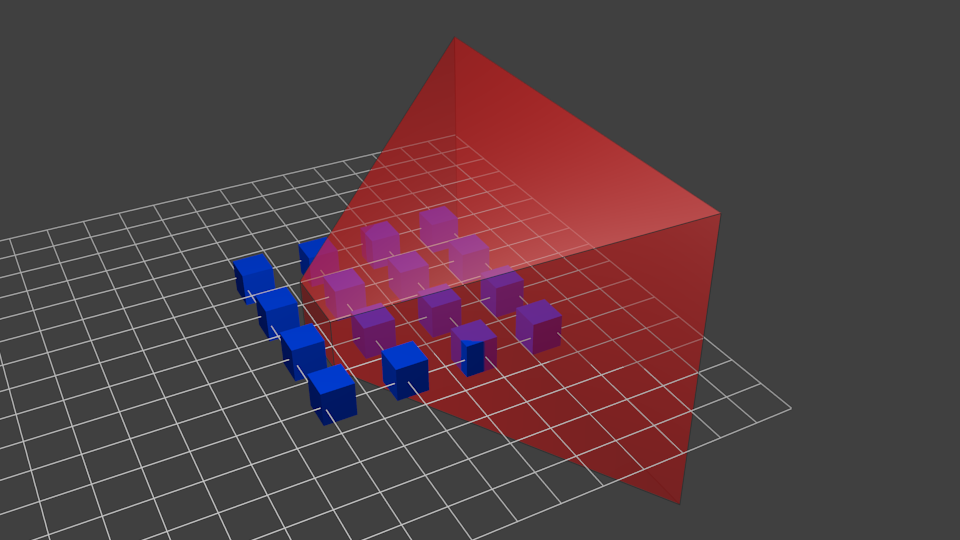
\includegraphics[width=0.6\textwidth]{images/frustum/frustum_cubes.png}
\caption{Il frustum prima della trasformazione.\label{example1}}
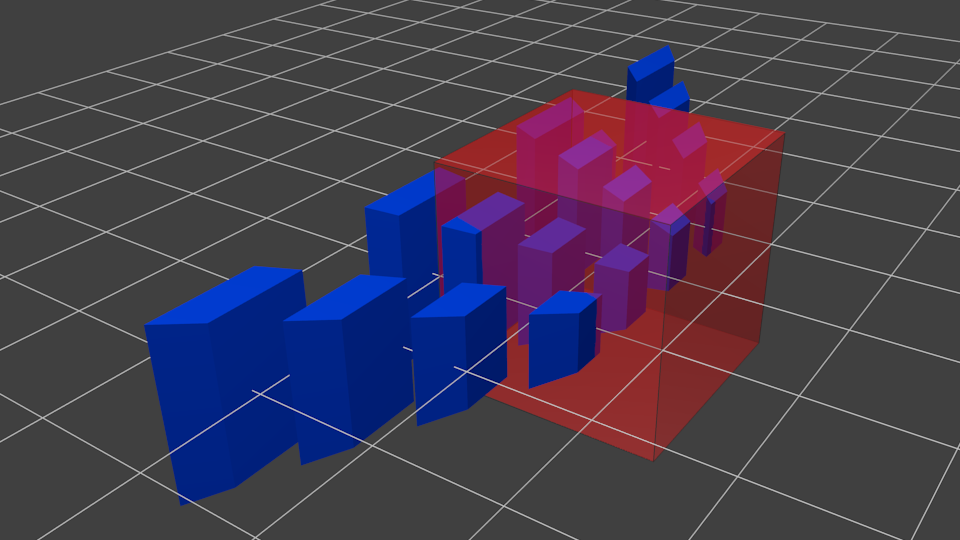
\includegraphics[width=0.6\textwidth]{images/frustum/frustum_homogeneous.png}
\caption{Il frustum trasformato nel sistema di coordinate normalizzato.\label{example2}}
\end{figure}

Nella figura \ref{example3} il cubo è visto dal suo piano frontale.

\begin{figure}[htbp]
\centering
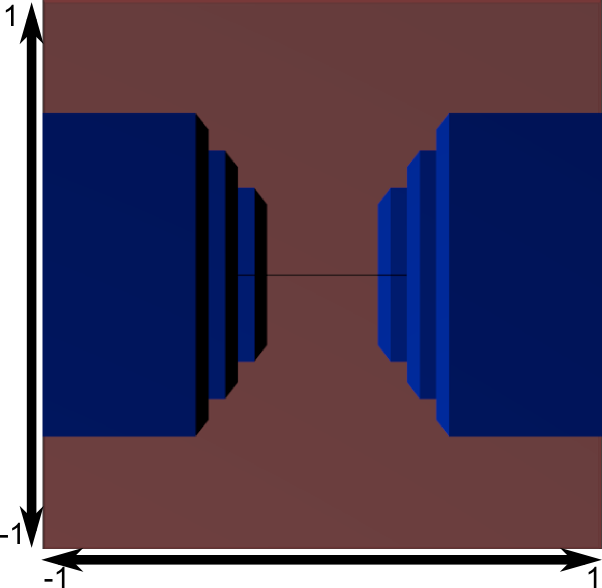
\includegraphics[width=0.5\textwidth]{images/frustum/frustum_view.png}
\caption{Il nuovo frustum visto in prospettiva.\label{example3}}
\end{figure}

La matrice $4\times 4$ \footnote{Il sistema utilizzato è detto di coordinate omogenee, sistema introdotto intorno al 1837 da August Ferdinand Möbius\cite{homog}. Questo sistema prevede la rappresentazione di $N$ coordinate con vettori di $N+1$ dimensioni, ed è usato per descrivere i punti nella geometria proiettiva.} che rappresenta la proiezione prospettica è \footnote{Per la dimostrazione matematica che porta a questo risultato si può consultare il capitolo 5 del libro \cite{libro}}:

$$M_{persp}=
\begin{bmatrix}
\frac{2n}{r-l} & 0 & \frac{r+l}{r-l} & 0 \\
0 & \frac{2n}{t-b} & \frac{t+b}{t-b} & 0 \\
0 & 0 & -\frac{f+n}{f-n} & -\frac{2nf}{f-n} \\
0 & 0 & -1 & 0
\end{bmatrix}
$$

dove \textit{n} e \textit{f} sono le coordinate $z$ relative al near e far plane, \textit{l} e \textit{r} sono le $x$ relative al punto di congiunzione tra il near plane e, rispettivamente, left e right plane; \textit{b} e \textit{t} sono le $y$ relative al punto di congiunzione tra il near plane e, rispettivamente, bottom e top plane.

Ogni vertice $P$ viene trasformato nel vertice $P'$ grazie alla seguente moltiplicazione:
$$P'=M_{persp}\times P=
\begin{bmatrix}
P_x \\ P_y \\ P_z \\ 1
\end{bmatrix}$$

Il nuovo sistema (NDC) si dice normalizzato proprio perché i vertici vengono normalizzati tramite la divisione delle componenti per la loro quarta coordinata; infatti la coordinata $w$ di ogni vertice diventa uguale a 1. La porzione di spazio considerata (il cubo) ora prende il nome di Canonical View Volume.
%Nella projection matrix è compresa l'operazione che normalizza i vertici, mappando le coordinate in modo che siano comprese tra $-1$ e $1$. Questa normalizzazione è data da una divisione delle componenti di ogni vertice per la quarta componente, cioè la coordinata W.
%Per mappare le coordinate nell'intervallo di valori $\left[-1,1\right]$ le componenti di ogni vertice vengono divise per la quarta componente W.

%L'utilizzo della quarta coordinata per definire i vertici dà origine al sistema di coordinate omogenee. Questo sistema, introdotto da August Ferdinand Möbius intorno al 1837, prevede la rappresentazione di $N$ coordinate con vettori di $N+1$ dimensioni, ed è usato per descrivere i punti nella geometria proiettiva. Inoltre la quarta coordinata permette di rappresentare tutte le trasformazioni affini (trasformazioni lineari più una traslazione) tramite le matrici.
%
%Considerando che la traslazione di un vettore a due dimensioni $v = (x,y)$ per un vettore $v_0 = (a,b)$
%è data dalla loro somma, è possibile rappresentare questa trasformazione anche tramite una matrice $3\times3$:
%$$T_{v_0} \times v = \begin{pmatrix} 1 & 0 & a \\
%0 & 1 & b \\
%0 & 0 & 1
%\end{pmatrix}
%\begin{pmatrix}
%x \\
%y \\
%1 
%\end{pmatrix}
%=
%\begin{pmatrix}
%x + a \\
%y + b \\
%1
%\end{pmatrix}$$\\
%
%E' possibile estendere questo concetto ad ogni tipo di trasformazione, permettendo di raggruppare più trasformazioni in una singola matrice uguale al prodotto delle matrici che le rappresentano.

\subsubsection{View Matrix}
La Projection Matrix trasforma lo spazio considerando che la telecamera sia situata nell'origine e che la direzione dello sguardo sia rivolto lungo l'asse negativo delle Z. Per questo, se la telecamera è situata in punti diversi, si deve applicare un'altra trasformazione, che la porti nella sua posizione di default. Questa trasformazione è data dalla \textbf{View Matrix}, che ha il compito di trasformare lo spazio di coordinate del mondo 3D nello spazio di coordinate relativo alla telecamera. In pratica la telecamera viene ruotata e traslata per essere posizionata nell'origine, con il corretto orientamento, e nello stesso momento tutto il mondo 3D subisce la stessa trasformazione (figure \ref{view1} e \ref{view2}).

\begin{figure}[htbp]
\centering
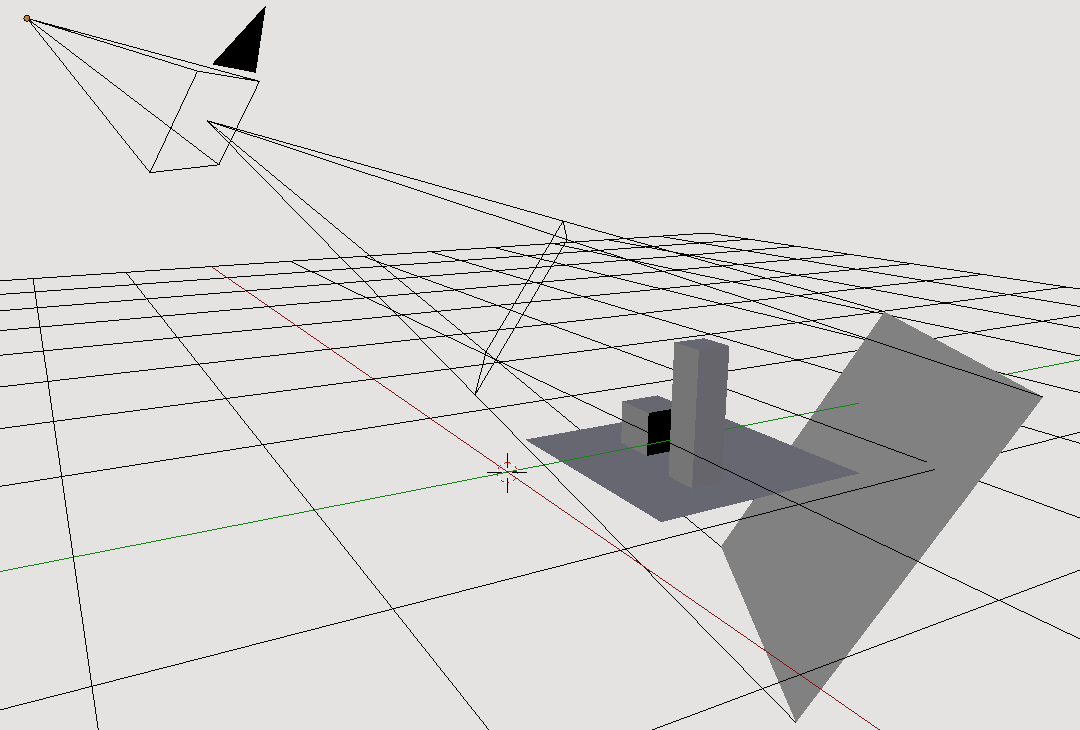
\includegraphics[width=0.9\textwidth]{images/frustum/view-before4-white2.png}
\caption{La telecamera è posta in un punto qualsiasi della scena.\label{view1}}
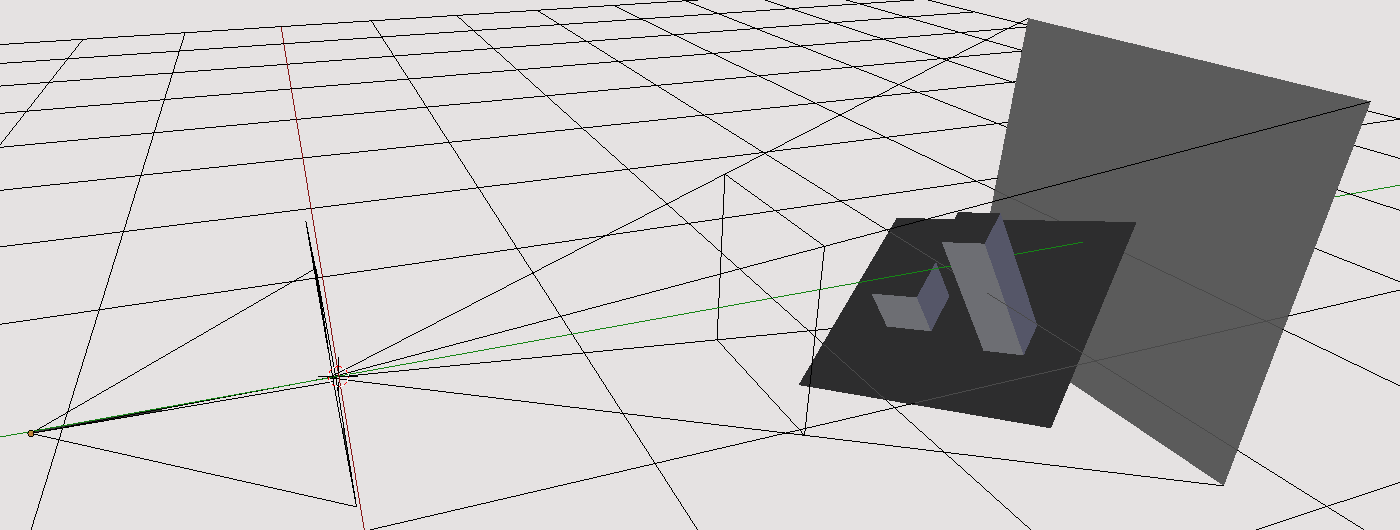
\includegraphics[width=0.9\textwidth]{images/frustum/view-after4-white2.png}
\caption{La scena trasformata tramite la view matrix, in modo da posizionare la telecamera nella sua posizione di default.\label{view2}}
\end{figure}


Dopo aver applicato questa trasformazione è possibile applicare anche la proiezione.

Il calcolo della View Matrix necessita di tre vettori:
\begin{itemize}
\item \textbf{eye}: identifica la posizione della telecamera.
\item \textbf{target}: identifica il punto verso cui è rivolto lo sguardo.
\item \textbf{up}: identifica la direzione che punta verso l'alto, di solito coindice con l'asse y, quindi è $(0, 1, 0)$.
\end{itemize}

La matrice consiste in due trasformazioni: una rotazione, per allineare l'orientamento della telecamera con l'asse negativo delle Z, e una traslazione, per spostare la telecamera nell'origine.
Per la rotazione si calcola una base ortonormale che rappresenta il sistema di coordinate relativo alla telecamera (figura \ref{cam-axis}), tramite i tre vettori, ponendo
\begin{lstlisting}
n = normalize( eye - target );
u = normalize( cross( up,n ) );
v = cross( n,u );
\end{lstlisting}
dove $cross(a,b)$ rappresenta il prodotto vettoriale tra $a$ e $b$ e $normalize(a)$ la normalizzazione di $a$. I vettori $u$,$v$,$n$ formano la base ortonormale desiderata.

\begin{figure}[htbp]
\centering
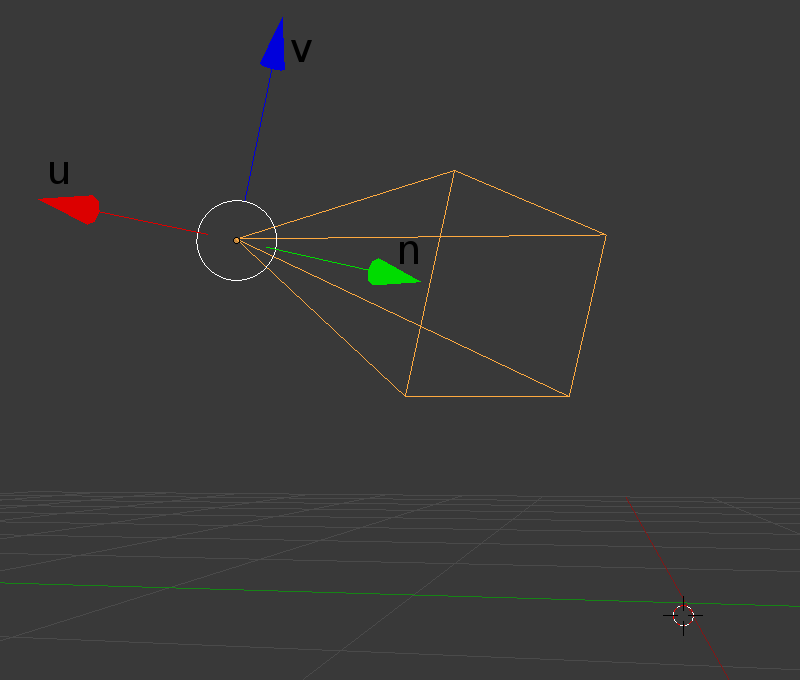
\includegraphics[width=0.6\textwidth]{images/frustum/camera-axis.png}
\caption{Il sistema di coordinate relativo alla telecamera.\label{cam-axis}}
\end{figure}

La View Matrix finale è la seguente:

$$V=
\begin{bmatrix}
u.x && u.y && u.z && -dot( u, eye )\\
v.x && v.y && v.z && -dot( v, eye )\\
n.x && n.y && n.z && -dot( n, eye )\\
0 && 0 && 0 && 1\\
\end{bmatrix}
$$\\
dove $dot(a,b)$ rappresenta il prodotto scalare tra $a$ e $b$.


\subsubsection{Viewport Matrix}
L'ultimo passaggio è dato dalla \textbf{Viewport Matrix}, che trasforma i vertici dal sistema di coordinate normalizzato, al sistema di coordinate relativo allo schermo. Dopo questa fase, il nuovo sistema di riferimento è relativo all'angolo in basso a sinistra della finestra aperta dopo aver lanciato l'applicazione, e le coordinate sono date dai pixel dello schermo.

Dati i valori \textit{w} (width = larghezza) e \textit{h} (height = altezza), in pixel, il canonical view volume viene ridotto, scalandolo di $w/2$ nella direzione orizzontale e di $h/2$ nella direzione verticale. Dopo di ciò il tutto viene traslato di un vettore $(-w/2, -h/2, -1)$ per allineare l'angolo in basso a sinistra di fronte del canonical view volume (cioè il punto $(-1,-1,-1)$) con l'angolo in basso a sinistra della finestra visualizzata a schermo.

Tutte le operazione che si svolgono dopo, come la rasterizzazione e lo shading, vengono fatte usando questo sistema di riferimento.

\clearpage